\chapter{主な機能}\label{chap:features}

前章で宣言した通り,本論文で防ぎたいコンパイルエラーの種類は以下の3つである.
\begin {itemize}
  \item シンタックスエラー
  \item 型エラー
  \item Unbound valueエラー
\end {itemize}

シンタックスエラーについては,穴のないブロックであれば,ブロックと構文木が一対一対応しているために起き得ない.変数名にキーワードが使えないようにする必要もあるが,その対処も行うこととする.
型エラーについては,ブロックの各コネクタに型表現を割り振るという第\ref{chap:senko}章で述べた\cite{Typed-Blockly}のアイデアを参考にして,
let多相や型の単一化のリセット機能を実装し,型推論を拡張する.
接続させると型推論が失敗するようなコネクタをユーザが接続させようとしたら,ブロックの接続を拒絶すればよい.
最後に,Unbound valueエラーを防ぐために,変数ブロックの生成や,変数ブロックを含んだブロックのスコープを管理する.
上に示した3つ以外を理由としたコンパイルエラーについては,第\ref{chap:todo}章にて議論する.

本研究で行った主な実装のうち,以下の4つの機能をそれぞれ画像を交えて説明する.
\begin {enumerate}
  \item 変数束縛
  \item スコープお砂場
  \item let多相を含んだ型システム
  \item メッセージ出力
\end {enumerate}
実装方法については,次章にてそれぞれ詳しく説明する.

\section {変数束縛}

変数スコープや変数束縛の関係は,関数型言語初学者にとって,理解しにくいものの1つと言える.
多くの命令型言語では,変数宣言文と同列にある閉じ括弧{\tt \}}が出現するまでの文がスコープとなるのに対し,
関数型言語では,OCamlやHaskellのletのように,in内の式が終了するまでがスコープとなる.
このようなスコープの概念に馴染みの無い初学者は,例えば「{\tt (let foo = ...\ in ?); foo}」のような,
スコープ外で{\tt foo}にアクセスするようなミスをしがちである.

初学者がOCamlにおけるスコープの概念を理解しやすいように,変数参照は必ず変数宣言から生成させる.
これによって未定義の変数を参照することが原理的に起きえなくなる.
また,一度生成した変数参照はその参照先を配置された位置によって変えない.
これによりユーザの想定していなかったシャドウイングによってプログラムの意図が変わることを防ぐ.
変数参照を表す変数参照ブロックを以降,単に「変数ブロック」と呼ぶ.
変数ブロックの生成の流れを図\ref{fig:boundFoo}に示し,
変数ブロックをドラッグしたときの様子を図\ref{fig:refBlockFoo},\ref{fig:dupFoo}に示した.

例えば,図\ref{fig:refBlockFoo}でユーザが組み立てようとしているプログラムは,左から順に「{\tt (let foo = ?\ in ?); foo}」,「{\tt let foo = foo in ?}」,「{\tt let foo = ?\ in foo}」であるが,初めの2つはプログラムとして正当でない.よって,ドラッグ中のブロック全体を不透明にして,目的の位置にブロックを移動できないこと,あるいは目的のコネクタにブロックを接続できないことをユーザに伝える.

図\ref{fig:dupFoo}は,ユーザがどこから変数ブロックを生成したかによって変数ブロックの扱いが異なることを示した例である.
組み立てようとしているプログラムはどちらも「{\tt let foo = ?\ in let foo = ?\ in foo}」であり,
OCamlのプログラムとしてはどちらも正当だが,
ユーザが意図した変数を正しく参照することのできない左のケースでは,コネクタとの接続を拒否する.

なぜそこにブロックを置くことができないのか,接続できないのかといった理由を説明したエラーメッセージの出力も行っており,
これについては第\ref{fun:message}節にて紹介する.
% 段落切り替えがなぞ

正しく束縛されない変数ブロックが存在したままユーザがその場にブロックを落とした場合は,
ブロックが生成されたばかりならばブロックを削除し,そうでないならドラッグ開始前の位置,状況に戻らせる.
また,変数をホバーしたときに関連した全ての変数がハイライトされるようになっており,
束縛関係を把握しやすいようになっている(図\ref{fig:dupFooHover}).
スコープに従ったアルファ変換(変数名の変更)も行うことができる.

\begin{figure}[H]
 \centering
 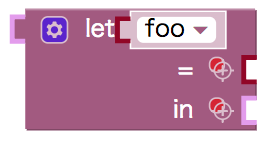
\includegraphics[keepaspectratio, scale=0.3]{img/boundFoo0.png}
 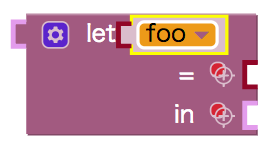
\includegraphics[keepaspectratio, scale=0.3]{img/boundFoo1.png}
 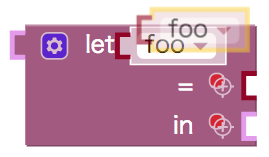
\includegraphics[keepaspectratio, scale=0.3]{img/boundFoo2.png}
 \caption{変数ブロックを生成する流れ.変数宣言を囲うように描画されたブロック(左)にカーソルを合わせて(中)ドラッグする(右)と,
変数ブロックの生成を行うことができる.\label{fig:boundFoo}}
 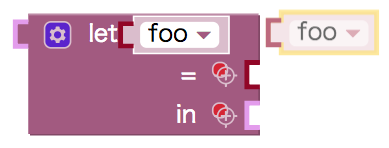
\includegraphics[keepaspectratio, scale=0.3]{img/refBlock0.png}
 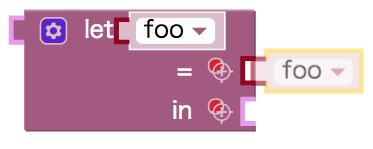
\includegraphics[keepaspectratio, scale=0.3]{img/refBlock1.png}
 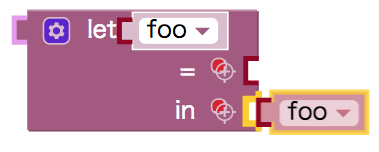
\includegraphics[keepaspectratio, scale=0.3]{img/refBlock2.png}
 \caption{変数ブロック「{\tt foo}」を生成後にドラッグしたまま動かしたときのブロックの様子.
正しく変数ブロックが束縛されない場合はブロックを不透明に表示する.\label{fig:refBlockFoo}}
 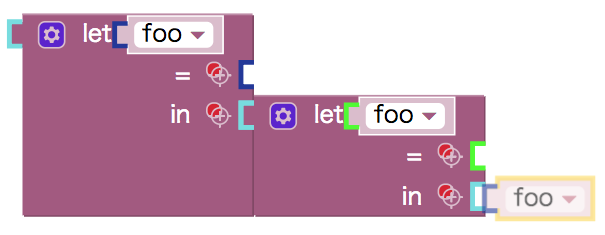
\includegraphics[keepaspectratio, scale=0.3]{img/dupFoo0.png}
 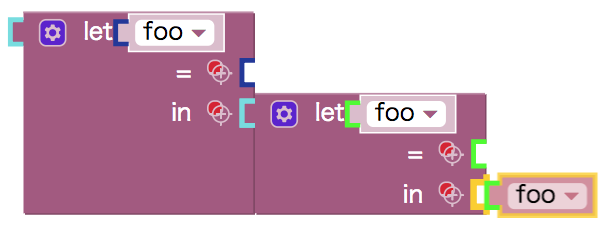
\includegraphics[keepaspectratio, scale=0.3]{img/dupFoo1.png}
 \caption{外側の変数宣言部分から生成した変数ブロック(左)と,
内側から生成した変数ブロック(右)を内側のin以下に接続させようとしたときの比較.
変数ブロックのコネクタの色にも注目されたい.\label{fig:dupFoo}}

 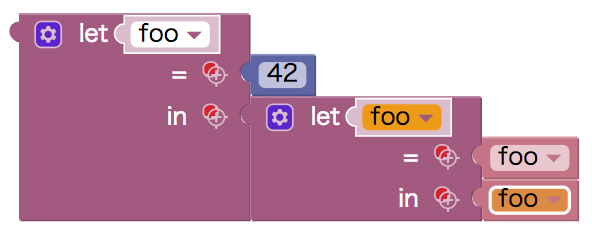
\includegraphics[keepaspectratio, scale=0.3]{img/dupFooInt42.png}
 \caption{右下の変数ブロックをホバーしたときの反応.束縛変数,
束縛されている変数がオレンジ色にハイライトされる.\label{fig:dupFooHover}}
\end{figure}
\clearpage

\section {スコープお砂場}

変数ブロックや変数ブロックを含むブロックをスコープが有効な場所にしか置けないという制約を設けると,ブロックを自由な場所に置き,好きな順番でブロックを組み立てられるという,Blocklyにあった利点を損なってしまう.これを避けるため,本研究では,スコープチェックのついた遊び場を設け,これを「スコープお砂場」と命名した.使用例を図\ref{fig:osunaba}に示す.

\begin{figure}[H]
 \centering
 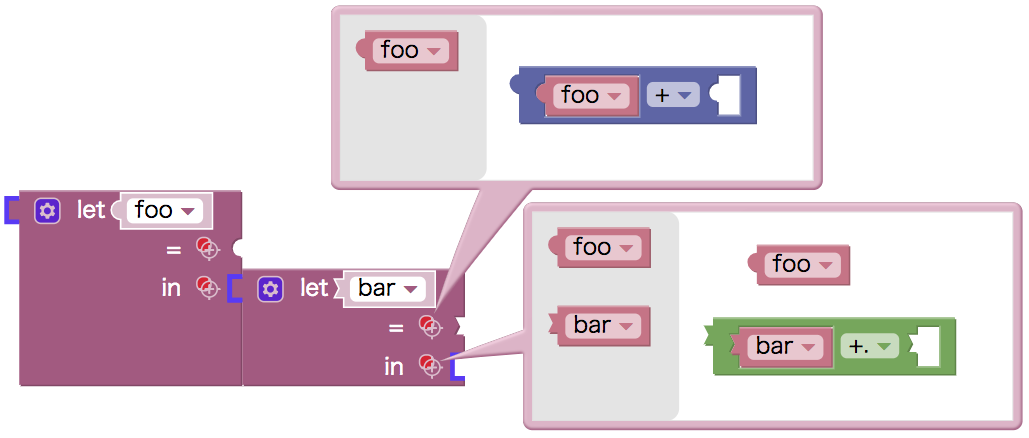
\includegraphics[keepaspectratio, scale=0.3]{img/osunaba3.png}
 \caption{スコープお砂場の例.ブロック上の赤いアイコンをクリックするとポップアップが現れる.スコープで参照できる変数ブロックの一覧を持つサイドメニューが左側に見れ,ブロックの生成が行える.スコープお砂場内で,変数ブロックをどんな型として扱うかによって,変数宣言のブロックの型も変化する.\label{fig:osunaba}}
\end{figure}

スコープお砂場は新しい変数が加わりうる各入力コネクタに紐づいており
\footnote[2]{図\ref{fig:osunaba}では,inの直前のスコープにもお砂場のためのアイコンが表示されているが,これはletに引数を追加する場合やrecフラグを有効にした場合に必要になる.},
コネクタの隣にあるアイコンをクリックするとポップアップの形で表示される.
スコープお砂場にはフライアウトメニューが付いており,そこには所属先のコネクタから参照できる変数の一覧が並んでいる.その変数ブロックをドラッグすることで,ブロックの生成も行える.
ユーザはこのスコープお砂場でブロックを適当に組み合わせたのち,目的のブロックと接続をすればよい.
スコープお砂場は,入れ子にしても使うことができる.

このお砂場にはスコープチェックがついており,所属先のコネクタから参照することができない変数を含むブロックはお砂場に移動することができない.例えば図\ref{fig:osunaba}の右下のお砂場にある「{\tt foo}」ブロックはもう一方のお砂場に移動できるが,「{\tt bar +.\ ?}」のブロックは移動することはできない.ブロックが不透明になり,ブロックをそのままリリースしてもブロックの移動はキャンセルされる.

また,お砂場を所有するブロックが移動する際は,お砂場内のブロックもスコープチェックの対象である.
例えば,図\ref{fig:osunaba}の「{\tt let bar = ?\ in ?}」を表すブロックを動かして「{\tt let foo = ?\ in ?}」の2つ目のスコープから外した場所に置くことはできない.
お砂場内に変数ブロック「{\tt foo}」が存在しているためである.

% 一番大変だったわりに説明がすくねえ

\section {let多相を含んだ型システム}

let多相を含む型システムを実装した.
また,型の単一化の解除をサポートした.例えば,リストコンストラクタのブロック「{\tt ?\ ::\ ?}」に{\tt int}型ブロックを入れて「{\tt 3 ::\ ?}」とすると,出力コネクタが{\tt 'a list}から{\tt int list}を表す形に変わるが,{\tt int}型ブロックを外すと{\tt 'a list}の形に戻る.

同じ変数の型は,例えば図\ref{fig:osunaba}の変数「{\tt bar}」のように,スコープお砂場に置かれたブロックであっても一貫していなければならないとした.
例えば,スコープお砂場の外で宣言された変数を参照する変数ブロックが,
スコープお砂場内で{\tt float}型として扱われたならば,元の変数宣言も{\tt float}型であると決定される.

\section {メッセージ出力\label{fun:message}}

不正なプログラムを組み立てられないユーザインタフェースを設けると,
なぜ不正なのかをまだ理解できない初学者が困惑してしまう可能性があり,
本研究が達成するべき「理解しやすさ」が不十分になってしまう.
これを回避するため,本システムではドラッグ中のエラーを書いたツールチップの表示を行った(図\ref{fig:errorOutput}).
なぜユーザの意図した場所にブロックを置くことができないのか,なぜ目的のブロックと接続できないのかといった理由を見ることができる.

\begin{figure}[h]
 \centering
 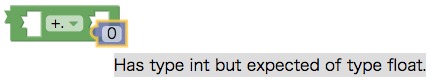
\includegraphics[keepaspectratio, scale=0.4]{img/errorIntFloat.png}
 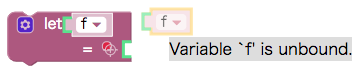
\includegraphics[keepaspectratio, scale=0.4]{img/errorUnbound.png}
  \includegraphics[keepaspectratio, scale=0.4]{img/errorDupVar2.png}
 \caption{エラーツールチップの例.\label{fig:errorOutput}}
\end{figure}

